\documentclass[12pt,twoside,titlepage]{report}

%%%%%%%%%%%%%%%%%%%%%%%%%%%%%% Paquetes %%%%%%%%%%%%%%%%%%%%%%%%%%%%%%%%%%%%%

\usepackage[a4paper,bindingoffset=3mm,bottom=35mm]{geometry}
\usepackage[colorlinks=true,pdftex]{hyperref}   %%% Opcional. Para incluir marcadores y enlaces en el pdf
\usepackage[pdftex]{graphicx}  %%% para pdflatex. Las figuras pueden estar en pdf, jpg, svg y otros formatos
\usepackage[spanish]{babel}
%\usepackage[latin1]{inputenc} % Usad en WinEdt/MikTex
\usepackage[utf8]{inputenc} % Usad en overleaf
%\usepackage[T1]{fontenc}
\usepackage{amsmath,amssymb}
\usepackage{hyperref}
\usepackage{color}
\usepackage{afterpage}
\usepackage{paralist}
\usepackage{array}
\usepackage{enumerate}
\usepackage{paralist}
\usepackage{enumitem}
\usepackage{float}
\usepackage{setspace}
\usepackage{listings}
\usepackage{algorithm}
\usepackage{algorithmic}
\usepackage{fancyhdr}
\usepackage{rotating}
\usepackage{multirow}
\usepackage{quotchap}
\usepackage{lipsum}
\usepackage{verbatim} % comentarios

%%%%%%%%%%%%%%%%%%%%%%% Definiciones básicas %%%%%%%%%%%%%%%%%%%%%%%%%%%%%%%

\newcommand{\nombreautor}{Alberto Gómez Cano}
\newcommand{\nombretutor}{Manuel Rubio Sánchez}
\newcommand{\titulotrabajo}{EARFIT: Aplicación Para Entrenamiento Auditivo Musical}
\newcommand{\escuela}{Escuela Técnica Superior\\de Ingeniería Informática}
\newcommand{\escuelalargo}{Escuela Técnica Superior de Ingeniería Informática}
\newcommand{\universidad}{Universidad Rey Juan Carlos}
\newcommand{\fecha}{\today}
\newcommand{\grado}{Grado en Ingeniería Informática}
\newcommand{\curso}{Curso 2021-2022}
\newcommand{\logoUniversidad}{logoURJC.pdf}
\graphicspath{ {assets/} }


% Definiciones de colores (para hidelinks)
\definecolor{BlueLink}{rgb}{0.165,0.322,0.745}
\definecolor{PinkLink}{rgb}{0.8,0.22,0.5}
\definecolor{gray}{rgb}{0.6,0.6,0.6}
% Enlaces
\hypersetup{hidelinks,pageanchor=true,colorlinks,citecolor=PinkLink,urlcolor=black,linkcolor=BlueLink}
\newcommand\blankpage{%
    \newpage
    \null
    \thispagestyle{empty}%
    %\addtocounter{page}{-1}%
    \newpage}
% Texto referencias
\addto{\captionsspanish}{\renewcommand{\bibname}{Bibliografía}}
% Texto Índice de tablas
\addto\captionsspanish{\def\tablename{Tabla}\def\listtablename{\'{I}ndice de tablas}}
\floatname{algorithm}{Algoritmo}
\newfloat{algorithm}{t}{lop}
%\newenvironment{pseudocodigo}[1][htb]
%  {\renewcommand{\algorithmcfname}{Pseudocódig}% Update algorithm name
%   \begin{algorithm}[#1]%
%  }{\end{algorithm}}
  
%%%%%%%%%%%%%%%%%%%%%%% Estilo de código (en Python) %%%%%%%%%%%%%%%%%%%%%%%

\definecolor{bg}{rgb}{0.95,0.95,0.95}
\definecolor{mydeepteal}{rgb}{0.16,0.22,0.23}
\definecolor{myteal}{rgb}{0.31,0.44,0.46}
\definecolor{mymediumteal}{rgb}{0.41,0.58,0.60}
\DeclareFixedFont{\ttb}{T1}{txtt}{bx}{n}{12} % for bold
\DeclareFixedFont{\ttm}{T1}{txtt}{m}{n}{12}  % for normal
%\newcommand*{\FormatDigit}[1]{\textcolor{mydeepteal}{#1}}
\newcommand*{\FormatDigit}[1]{\textcolor{black}{#1}}
% Python style for highlighting
\newcommand\mypythonstyle{\lstset{
language=Python,
basicstyle=\ttfamily\small,
%basicstyle=\linespread{1.0}\footnotesize\ttm,
otherkeywords={self},             % Add keywords here
keywordstyle=\bfseries\ttfamily\color{myteal},
%keywordstyle=\ttb\color{myteal},
commentstyle=\itshape\color{myteal},
stringstyle=\color{mydeepteal},
emph={MyClass,__init__},          % Custom highlighting
emphstyle=\ttb\color{mydeepteal},    % Custom highlighting style
% Any extra options here
showstringspaces=false,            %
backgroundcolor=\color{bg},
rulecolor = \color{bg},
%identifierstyle=\color{deepgreen},
breaklines=true,
numbers=left,
numbersep=5pt,
numberstyle=\tiny,
tabsize=4,
xleftmargin=1em,
frame = single,
framesep = 3pt,
framextopmargin=0pt,
framexbottommargin=0pt,
framexleftmargin=0pt,
framexrightmargin=0pt,
fontadjust=true,
basewidth=0.55em, % compactness of code
upquote=true,
}}
% Python environment
\lstnewenvironment{mypython}[1][]
{
\mypythonstyle
\lstset{#1}
}
{}
\newcommand\mypythonstylenormalinline{\lstset{
language=Python,
basicstyle=\ttfamily\normalsize,
%basicstyle=\linespread{1.0}\footnotesize\ttm,
otherkeywords={self},            % Add keywords here
keywordstyle=\bfseries\ttfamily\color{myteal},
%keywordstyle=\ttb\color{myteal},
commentstyle=\itshape\color{mymediumteal},
stringstyle=\color{mydeepteal},
emph={MyClass,__init__},          % Custom highlighting
emphstyle=\ttb\color{mydeepteal},    % Custom highlighting style
% Any extra options here
showstringspaces=false,            %
backgroundcolor=\color{bg},
rulecolor = \color{bg},
%identifierstyle=\color{deepgreen},
breaklines=false,
numbers=left,
numbersep=5pt,
numberstyle=\tiny,
tabsize=4,
xleftmargin=0em,
frame = single,
framesep = 3pt,
framextopmargin=0pt,
framexbottommargin=0pt,
framexleftmargin=0pt,
framexrightmargin=0pt,
fontadjust=true,
%basewidth=0.55em, % compactness of code
upquote=true,
}}
\newcommand\mypythoninline[1]{{\mypythonstylenormalinline\lstinline!#1!}}

%%%%%%%%%%%%%%%%%%%%% Comandos definidos por el autor %%%%%%%%%%%%%%%%%%%%%%%%

\newcommand{\transpuesta}{\mbox{\tiny $\mathsf{T}$}}
 





%%%%%%%%%%%%%%%%%%%%%%%%%%%%%%%%%%%%%%%%%%%%%%%%%%%%%%%%%%%%%%%%%%%%%%%%%%%%%%
%                           Inicio del documento                             %
%%%%%%%%%%%%%%%%%%%%%%%%%%%%%%%%%%%%%%%%%%%%%%%%%%%%%%%%%%%%%%%%%%%%%%%%%%%%%%
 
\begin{document}
\pagestyle{plain}
  
%%%%%%%%%%%%%%%%%%%%%%%%%%%%%%%%%%%% Portada %%%%%%%%%%%%%%%%%%%%%%%%%%%%%%%%%%
 
% Universidad, Facultad
\begin{titlepage}
\selectlanguage{spanish}
 
% Logo
\begin{center}
\includegraphics[scale=0.7]{\logoUniversidad}
\end{center}
\bigskip
\begin{center}
\begin{LARGE}
\escuela \\
\end{LARGE}
\end{center}
\bigskip
\bigskip

% Grado
\begin{center}
\begin{large}
\textbf{\grado}\\
\end{large}
\end{center}

% Curso
\begin{center}
\begin{large}
\textbf{\curso}\\
\end{large}
\end{center}
\bigskip
\textbf{\begin{center}
\begin{large}
\textbf{Trabajo Fin de Grado}
\end{large}
\end{center}}
\bigskip
\bigskip
\bigskip

% Nombre del TFG
\begin{center}
\textbf{\begin{large}
\MakeUppercase{\titulotrabajo}\\
\end{large}}
\end{center}

% Nombre del autor y Tutor
\vspace{\fill}
\begin{center}
\textbf{Autor: \nombreautor}\\ \smallskip
\textbf{Tutor: \nombretutor}\\
\bigskip

% Fecha
%\textbf{\fecha}\\
\end{center}
\end{titlepage}

% Pagina en blanco
\hypersetup{pageanchor=true}
\normalsize
\afterpage{\blankpage}
 
% Estilo de párrafo de los capítulos
\setlength{\parskip}{0.75em}
\renewcommand{\baselinestretch}{1.25}

% Interlineado simple
\spacing{1}
\pagenumbering{Roman}
\setcounter{page}{2}

%%%%%%%%%%%%%%%%%%%%%%%%%%%%%%%%%%%%%%%%%%%%%%%%%%%%%%%%%%%%%%%%%%%%%%%%%%%%%%%%%%%

 
%%%%%%%%%%%%%%%%%%%%%%%%% Agradecimientos o dedicatoria %%%%%%%%%%%%%%%%%%%%%%%%%%%

\chapter*{Agradecimientos}

Quiero agradecer este TFG a mi familia por siempre estar a mi lado aconsejándome en los momentos más difíciles de mi carrera. 

A mi novia por aguantar mis frustraciones y animarme a seguir adelante. 

A mi tutor académico Manuel Rubio Sánchez que me ha apoyado para realizar este trabajo. 

Y finalmente, me gustaría agradecer a todos mis compañeros que han compartido esta carrera conmigo.

¡A todos, mil gracias!
\afterpage{\blankpage}

%%%%%%%%%%%%%%%%%%%%%%%%%%%%%%%%%%%%%%%%%%%%%%%%%%%%%%%%%%%%%%%%%%%%%%%%%%%%%%%%%%%

 
%%%%%%%%%%%%%%%%%%%%%%%%%%%%%%%%%%%% Resumen %%%%%%%%%%%%%%%%%%%%%%%%%%%%%%%%%%%%%%

\chapter*{Resumen}
Un gimnasio musical para tus oídos. La idea consiste en desarrollar una herramienta para ayudar a músicos a desarrollar su oído (Musical Ear Training). Por ejemplo, para identificar notas, intervalos, escalas, etc. Estos ejercicios mejorarán su capacidad musical al desarrollar una comprensión más intuitiva de lo que se escucha.

Además, este TFG tiene como objetivo centrarse en cómo crear un nuevo producto software desde cero. Siguiendo todas las etapas de desarrollo desde que se concibe la idea hasta que se obtiene el producto deseado. Con la idea en mente de plasmar los conocimientos adquiridos en los cuatro años de estudios pero también de aprender y usar diferentes tecnologías que estén a la orden del día. También se pretende hacer uso de la metodología Agile para llevar a cabo la organización del proyecto.

Consistirá en una aplicación web basada Next.js y TypeScript y que será desplegada en Vercel. Con el nombre de Earfit y que se puede visitar en el siguiente enlace:

\url{https://earfit-alberttogoca.vercel.app/}

\mbox{} \bigskip

% Palabras Clave
\noindent \textbf{Palabras clave}:
\begin{compactitem}
    \item Entrenamiento Auditivo
    \item Nextjs
    \item React
    \item TypeScript
    \item Vercel
    \item Agile
\end{compactitem}

\afterpage{\blankpage}

%%%%%%%%%%%%%%%%%%%%%%%%%%%%%%%%%%%%%%%%%%%%%%%%%%%%%%%%%%%%%%%%%%%%%%%%%%%%%%%%%%%

 
%%%%%%%%%%%%%%%%%%%%%%%%%%%%%%%%%%%% Índices %%%%%%%%%%%%%%%%%%%%%%%%%%%%%%%%%%%%

% Estilo de párrafo de los Índices
\setlength{\parskip}{1pt}
\renewcommand{\baselinestretch}{1}
\renewcommand{\contentsname}{Índice de contenidos}

% Índice de contenidos
\tableofcontents
\afterpage{\blankpage}

% Índice de figuras (OPCIONAL)
\listoffigures
\afterpage{\blankpage}
\addcontentsline{toc}{chapter}{\listfigurename}

% Índice de códigos/algoritmos (OPCIONAL).   El término "Códigos" se puede cambiar por "Métodos", "Funciones", "Algoritmos", etc.
\renewcommand\lstlistlistingname{Códigos}
\renewcommand\lstlistingname{Código}
\renewcommand\lstlistlistingname{Índice de códigos}

\lstlistoflistings
\afterpage{\blankpage}
\addcontentsline{toc}{chapter}{\lstlistlistingname}


%%%%%%%%%%%%%%%%%%%%%%%%%%%%%%%%%%%%%%%%%%%%%%%%%%%%%%%%%%%%%%%%%%%%%%%%%%%%%%%%%%%
  

%%%%%%%%%%%%%%%%%%%%%%% Cabeceras y pies de página (Opcional) %%%%%%%%%%%%%%%%%%%%%%%

%\setlength{\headheight}{15.2pt}
\pagestyle{fancy}
\renewcommand{\chaptermark}[1]{\markboth{Capítulo \thechapter.\ #1}{}}
\pagestyle{fancy}
\fancyhf{}
\fancyhead[LO]{\leftmark}
\fancyhead[RO]{}
\fancyhead[RE]{\nouppercase\rightmark}
\fancyhead[LE]{}
\fancyfoot[C]{\thepage}

%%%%%%%%%%%%%%%%%%%%%%%%%%%%%%%%%%%%%%%%%%%%%%%%%%%%%%%%%%%%%%%%%%%%%%%%%%%%%%%%%%%%

   
%%%%%%%%%%%%%%%%%%%%%%%%%%%%%% Capítulos de la memoria %%%%%%%%%%%%%%%%%%%%%%%%%%%%%


%%%%%%%%%%%%%%%%%%%%%%%%%%%%%% 1 Introducción %%%%%%%%%%%%%%%%%%%%%%%%%%%%%%%%%%%%%
\chapter{Introducción}

Si bien somos capaces de reconocer los colores desde bien pequeños, de forma general ponemos muy poco cuidado a los sonidos a lo largo de nuestra vida. Entrenar el oído es lo más parecido a aprender los colores y aprender cómo se relacionan y funcionan. Imagina un pintor que desconoce los colores, quién decide pintar el cielo morado porque no reconoce su verdadero color. En conclusión, un músico no puede darse el lujo de desconocer los colores de la música.

% Estilo resto de páginas
\pagestyle{fancy}

% Estilo de párrafo de los capítulos
\setlength{\parskip}{0.75em}
\renewcommand{\baselinestretch}{1.25}

% Interlineado simple
\spacing{1}

% Numeración contenido
\pagenumbering{arabic}
\setcounter{page}{1}

\section{Contexto}

Este apartado tiene como objetivo situar al lector. Por lo que daremos un poco de explicación sobre qué consiste el Entrenamiento Auditivo para que pueda comprender mejor el objetivo general y alcance del trabajo. También se realizará una pequeña descripción del proyecto y se comentará brevemente el estado del arte actual.

\subsection{Entrenamiento Auditivo}

Los oídos son la herramienta más importante a la hora de hacer música. Pero si no se entrenan, nunca desarrollarán toda su potencia.

Los músicos, productores y DJs se pueden beneficiar del entrenamiento de sus oídos. Puede resultar muy útil a la hora de mezclar música y componer canciones.

\subsubsection{Qué es}

El entrenamiento auditivo es el proceso de identificar los elementos de la música en su forma más sencilla y conectarlos con la forma en que sentimos el sonido físicamente. Tradicionalmente, el entrenamiento auditivo para los músicos incluye habilidades como identificar intervalos, tipos de acordes y progresiones de acordes. El entrenamiento auditivo para los productores de audio suele incluir la identificación de los rangos de frecuencias en Hz.

Muchas personas suponen que tener oído musical es tener la capacidad de identificar una nota al oírla. Tener oído musicales, también, ser capaz de escuchar y comprender música interiormente, sin que ésta este físicamente presente, igual que reflexionamos sobre palabras que hemos escuchado.

\subsubsection{Porqué es importante}

El entrenamiento auditivo es importante porque la escucha es una habilidad. Al igual que tocar el piano o saber cómo modificar una cadena de efectos vocales.

Por ejemplo, las melodías son simplemente series de intervalos. Con el entrenamiento necesario para identificar los intervalos, puedes aprender a tocar una melodía de oído.

Reconocer las progresiones de acordes de oído también es un superpoder. Acostumbrarse a escuchar las progresiones de acordes más comunes con una herramienta de entrenamiento auditivo cambia la forma en que compones canciones.

Al igual que tocar el piano o saber cómo modificar una cadena de efectos vocales, la escucha es una habilidad.
Para los productores de música, el entrenamiento auditivo sirve para identificar los rangos de frecuencias más rápidamente. ¿Quieres un kick más preciso? ¿O un vocal más ligero? El entrenamiento auditivo te ayudará a encontrar las frecuencias que necesitas para conseguir los efectos que buscas.

\subsubsection{Oído Absoluto}

Es la habilidad para reconocer notas musical sin tener otras como referencia. Es relativamente raro encontrar personas con oído absoluto. Se considera que menos del uno por ciento de la población tiene oído absoluto. Las posibilidades de tener oído absoluto aumentan si has recibido mucho entrenamiento musical desde muy pequeño.

\subsubsection{Oído Relativo}

Es la habilidad para reconocer notas musical relacionándolas entre sí. Es una habilidad indispensable para los músicos y es más sencilla de entrenar que el oído absoluto. Esta característica te puede permitir, por ejemplo, interpretar canciones sin disponer de partitura.

Las personas que disponen de oído relativo son capaces de:
\begin{itemize}
    \item Denotar la distancia de una nota musical desde una nota de referencia establecida.
    
    \item Seguir la notación musical, esto permite cantar correctamente una melodía entonando cada nota de acuerdo a la distancia con la nota anterior.
    
    \item Seguir la notación musical, esto permite cantar correctamente una melodía entonando cada nota de acuerdo a la distancia con la nota anterior.
\end{itemize}

Los ejercicios más comunes de entrenamiento auditivo te ayudarán a desarrollar tu oído relativo.

\subsubsection{Conclusión}

Aprender entrenamiento auditivo te lleva al siguiente nivel como músico ya que te permite sacar canciones más rápido, con mayor precisión, improvisarás mejor, podrás llevar al instrumento las melodías que imaginas con mayor facilidad, y en general te permitirá ser mucho mejor músico.

\subsection{Descripción del Proyecto}

El presente Trabajo de Fin de Grado se centra en el diseño e implementación de una aplicación web con la finalidad de ayudar a músicos a desarrollar su oído musical mediante la realización de ejercicios de entrenamiento auditivo. 

La aplicación se centrará en tres tipos diferentes de ejercicios divididos en la localización de notas, intervalos y escalas. 

Para cada uno de los ejercicios se ha diseñado una página específica, que incluirá:

El propio ejercicio, que consistirá en un botón que reproducirá el sonido correspondiente, calculado aleatoriamente teniendo en cuenta las posibles respuestas y los botones correspondientes a las respuestas a elegir. La idea es que el usuario trate de adivinar el sonido que está sonando. Cuando pulse en una respuesta se evaluará si es correcta o incorrecta. Si es incorrecta el botón cambiará a color rojo y podrá seguir probando. Si es correcta el botón cambiará a verde un segundo, se reseterán los botones y se calculará un nuevo sonido. También existe un contador de racha que aparecerá cuando se den tres aciertos consecutivos y desaparecerá cuando se falle.

A su derecha aparecerán las opciones con las que podrás personalizar el ejercicio a tu gusto, añadiendo o quitando respuestas del ejercicio lo que incrementará o disminuirá la dificultad. 

Además, en el ejercicio de notas se podrá cambiar la escala de la que se seleccionan las notas y en los ejercicios de intervalos y escalas se podrá elegir si las sucesión de notas será ascendente o descendente. 

También todos los ejercicios incorporarán un piano que los usuarios podrán usar para tocar notas de referencia y ayudarse en la obtención de la respuesta correcta. 

Aparte, se ha incorporado la posibilidad de poder cambiar el instrumento que suena y que será persistente para toda la aplicación.

Toda la aplicación se ha diseñado teniendo en mente que el diseño fuera simple, fácil de entender y limpio. Ha sido desarrollada utilizando Nextjs y Typescript que se explicarán más adelante en el apartado Implementación. Y se ha seguido un despliegue continuo de la aplicación en Vercel que también se explicará más adelante en Despliegue Continuo.

\subsection{Estado del Arte}
En la actualidad ya existen algunas aplicaciones para entrenar el oído como pueden ser:

ToneGym: \url{https://www.tonegym.co/}

ToneDear \url{https://tonedear.com/}

EarMaster: \url{https://www.earmaster.com/es/}

La mayoría de ellas está de acuerdo en qué el método más efectivo para progresar en el entrenamiento auditivo es el siguiente:

\begin{itemize}
    \item Aumentar la frecuencia que se practica, no la duración. Esto se debe a que, después de haber pasado un tiempo practicando, el cerebro continúa pensando en ello y haciendo nuevas conexiones neuronales en segundo plano, incluso mientras se duerme (especialmente mientras se duerme). Por esta razón, se recomienda marcar tus ejercicios favoritos y hacerlos todos los días durante un tiempo determinado.
    
    \item Empezar de forma simple y aumentar gradualmente la dificultad. La práctica debe ser un desafío, pero no tanto como para sentirse abrumado.
    
    \item Realizar un seguimiento del progreso. Tener en un cuaderno, un archivo de texto o incluso una hoja de cálculo con el seguimiento del progreso. Esto permite saber con certeza si se está mejorando. Si puedes ver tu mejora, te alentará a continuar. También puede ayudar anotar cuándo se está estancado para poder encontrar la causa. Quizá no practicas con la suficiente frecuencia o aumentaste la dificultad demasiado rápido.
    
    \item Cantar escalas e intervalos. Todos los ejercicios de estos sitios implican identificar notas en lugar de generarlas, pero eso no significa que no debas cantar junto con ellas. Esto ayuda a internalizar los tonos. Es especialmente útil para el ejercicio de escalas. Intentar cantar hacia arriba y hacia abajo todas las escalas te ayudará a interiorizarlas.
    
    \item Transcribir música con un instrumento. Elegir tus canciones favoritas e intentar descubrir las notas con un instrumento es una buena práctica. Puedes comenzar con la melodía y luego intentar descifrar los acordes, o puedes empezar con los acordes y luego intentar descifrar la melodía. Practica en ambos sentidos.
\end{itemize}

Todas ellas plantean diferentes ejercicios para reconocer notas, intervalos y escalas. La mayor diferencia que se encuentra en ellas es su diseño y su nivel de personalización de los ejercicios, que es donde vamos a enfocar este trabajo. Dando no sólo una aplicación con ejercicios sino una herramienta que te dé la libertad de configurarla a tu gusto.

\section{Objetivos}

El objetivo principal del TFG es desarrollar una herramienta que permita ayudar a músicos a desarrollar su oído musical. Mediante el entrenamiento auditivo.

Otros objetivos son:
\begin{compactitem}
    \item Utilizar nuevas tecnologías que estén a la orden del día
    \item Utilizar metodologías Ágiles
    \item Realizar un despliegue continuo de la aplicación
\end{compactitem}

\section{Estructura del documento}

En este apartado se especificará, como su título indica, la estructura que plantea este breve trabajo o memoria. El objetivo de dicho punto es acercar al lector las diferentes partes que componen este proyecto, así como ayudarle en la comprensión de este.

Se espera que sea lo suficientemente clarificador y que permita una lectura comprensible, rápida y amena del trabajo que nos ocupa.

\begin{itemize}

    \item En el Capítulo 1: Introducción, hemos realizado una pequeña puesta en contexto y explicación de los objetivos de este TFG. Además hemos explicado en qué consiste el Entrenamiento Auditivo y porqué es importante. A parte de una breve descripción del proyecto.
    \item En el Capítulo 2: Contenidos Principales, se explicará cómo ha sido el desarrollo de la aplicación.
    
    Empezando por Creación de Propuesta, donde exploraremos el concepto de Cómo nace la Idea aplicando Lean Startup, Design Thinking y diferentes métodos utilizados en esta fase, desde que surge la idea hasta el primer prototipo.

    Más tarde en Metodología de Trabajo se explicará la metodología que se ha seguido día a día a la hora de realizar la aplicación, hablaremos de Scrum y DevOps. Cómo se ha realizado la Integración Continua CI con Github y el Despliegue Continuo CD con Vercel.
    
    Luego, en Desarrollo e Implementación se trataran las Tecnologías Empleadas cómo Next.js o TypeScript entre otras. 
    
    Se detallará el diseño y un análisis de cómo funciona la aplicación por dentro en el apartado Implementación y cómo se ha verificado su funcionamiento en Testing. 
    
    Finalmente, se mostrará el resultado final de todo este proceso.
    \item Por último, en el Capítulo 3: Conclusiones, se detallan las conclusiones derivadas del trabajo, lo qué he aprendido, y lo que queda por mejorar.

\end{itemize}

% \afterpage{\blankpage} % puede generar problema en índice de contenidos
% \newpage


%%%%%%%%%%%%%%%%%%%%%%%%%%%%%% 2 Contenidos Principales %%%%%%%%%%%%%%%%%%%%%%%%%%%
\chapter{Contenidos principales}
\label{chap:contenidos}

\section{Creación de la Propuesta de Valor}

\textbf{¿Cómo nace la idea?}

La idea parte de la necesidad de jóvenes músicos que quieren aprender a tocar un instrumento. Una parte fundamental del aprendizaje consiste en entrenar el oído, que sin los medios adecuados puede resultar difícil.

Junto con mi tutor Manuel Rubio, que es un apasionado de la música, intentamos dar forma a esta solución. Tuvimos varias reuniones en las que él, cómo músico, me explicaba las dificultades por las que pasan a la hora de entrenar el oído. Una vez tenidas claras sus necesidades era hora de crear una solución que aportase valor. Para ello decidí crear un producto mínimo viable (\textbf{MVP}) que cumpliese con las especificaciones requeridas usando \textbf{Lean Startup}, como método de aprendizaje validado y \textbf{Design Thinking}, como método de generación de ideas innovadoras.

Aplicando las bases de Lean Startup combinándolas con prácticas de Design Thinking \textbf{(Lean Design)}, como se explica a continuación, se consiguió desarrollar un MVP.

\subsection{Lean Startup}
\subsubsection{Qué es}
Es un método riguroso para agilizar la puesta en marcha de soluciones y optimizarlas con base en un proceso de aprendizaje y de corrección iterativa. Comenzó con el método de desarrollo de clientes y el método Lean en los sistemas de fabricación japoneses popularizado por Toyota.

Se compone de 5 principios básicos:
\begin{enumerate}
    \item Los emprendedores están en todas partes
    \item El espíritu emprendedor es management
    \item Aprendizaje validado
    \item Crear medir aprender
    \item Contabilidad de la innovación
\end{enumerate}

\subsubsection{Porqué he decidido usarlo}

El Lean Startup \textbf{sirve para} acortar los ciclos de desarrollo, medir el progreso y ganar feedback por parte de los usuarios. Esto se consigue porque se basa en el \textbf{aprendizaje validado}, la \textbf{experimentación científica} y la \textbf{iteración} en los lanzamientos del producto. 

Aunque por su nombre pueda parecer que sólo esta enfocado al mundo Startup y crear una nueva empresa, en realidad es una herramienta imprescindible para la puesta en marcha de \textbf{soluciones software} como veremos a continuación.

\subsubsection{Explicación Detallada}

Para entender mejor el por qué de usar este método, explicaremos las \textbf{3 partes} de las que se compone y que hemos seguido, añadiendo prácticas de \textbf{Design Thinking} para la construcción de nuestra solución. Lo cual ayudará a entender el proceso que se ha seguido hasta llegar al resultado final:


\begin{figure}[H]
    \centering
    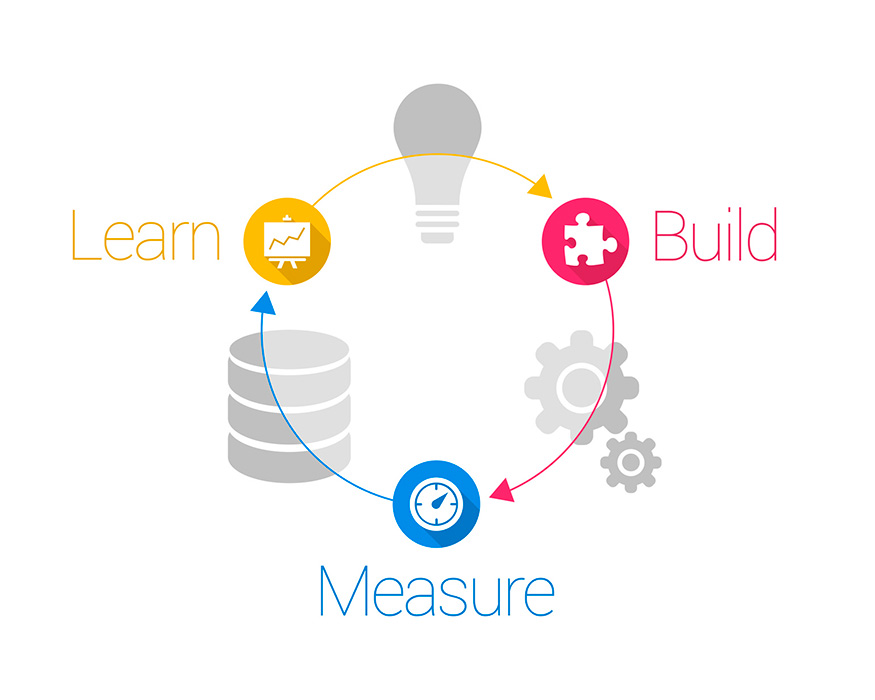
\includegraphics[scale=0.3]{leanstartup}
    \label{fig:Circuito de feedback de informacion}
\end{figure}

\subsubsection{1. VER}

\textbf{Comenzar}

El objetivo es conocer qué quieren los potenciales usuarios. 

Las startups se caracterizan por su constante incertidumbre. Así que en vez de hacer planes concretos apuntando a una sola dirección deben recoger feedback de sus potenciales clientes y hacer ajustes con la información que van recogiendo. Esto se llama \textbf{Circuito de feedback de información: crear, medir, aprender.}

\textbf{Definir}

Diseñar para crear un nuevo producto o servicio bajo condiciones de incertidumbre extrema. Un emprendedor no es sólo el fundador de una startup, también pueden ser managers de grande compañías creando nuevos negocios, o como es nuestro caso el lanzamiento de una nueva solución software.

Bajo estas condiciones de \textbf{incertidumbre} extrema las herramientas tradicionales de management no pueden funcionar bien. \textbf{Por eso necesitamos Lean Startup}.

\textbf{Aprender}

La función más importante de una startup es aprender qué quieren realmente los consumidores y que llevaría a un negocio sostenible. Para ello se necesita un proceso con disciplina de aprendizaje, lo que se llama \textbf{aprendizaje validado}. 

Se trata de tener hipótesis testeables y diseñar experimentos para testearlas, luego analizar los datos para así aprender de ellos.

\textbf{Experimentar}

La metodología Lean Startup ve el hecho de crear una startup/producto como una ciencia. Crear una \textbf{hipótesis}, diseñar un \textbf{experimento} para \textbf{testear} esa hipótesis, llevar a cabo el experimento, reunir datos, reflexionar y ver si validan o rechazan la hipótesis.

Las hipótesis deberían girar entorno al problema más importante de una startup, cómo construir un negocio sostenible alrededor de tu visión. O en nuestro caso cómo construir una solución que realmente aporte valor.

Según Lean Startup la mejor forma es trackeando el comportamiento de gente real y no preguntar por opiniones ya que a veces no son capaces de verbalizar lo que quieren.

Por ello hay que pensar en el experimento más barato y rápido para validar la hipótesis, lanzarlo pronto dará más información del comprador antes de lanzar el producto real. Sobre si están interesados o no en lo que estás construyendo y te hace ver preocupaciones de estos que no tenias cuantificadas.

\subsubsection{2. DIRIGIR}

Qué tan rápido puedes desarrollar tus experimentos.

Primero estableces tu hipótesis, luego construyes tu \textbf{producto minimo viable (MVP)} para testear esa hipótesis. Luego llevas a cabo el experimento, lo más común es poner los usuarios delante del producto y recoger así información sobre su comportamiento. Recoges los datos y reflexionas sobre ellos para seguir adelante o cambiar de dirección. 

Cuanto más rápido te muevas en este circuito, más rápido aprendes.

\textbf{Saltar}

Normalmente hay 2 tipos de hipótesis: hipótesis de creación de valor e hipótesis de crecimiento. Algunas hipotesis son más arriesgadas que otras. Unas tienen muchas probabilidades de ser ciertas y otras mucho menos. Las que tienen más riesgo son similares a las siguientes: 

¿Tiene la gente el problema que crees que tienen?

¿Realmente quieren lo que estas ofreciendo?

¿Pagarían por ello?

Un marco para empezar una startup es por analogía si alguien ha tenido éxito con un modelo de negocio si realizamos el mismo modelo de negocio con un servicio distinto también debería tener éxito. Esta idea puede parecer perfecta pero por otro lado esconde algunas presunciones sobre como funcionará el negocio. Para poder hacer una buena analogía hay que detallarla mucho más.

Hay muchas asunciones a tener en cuenta antes de construir tu prototipo por analogía. Lean Startup habla de una técnica utilizada en la fabricación japonesa llamada Genchi Genbutsu-“Go and See” que sería algo como ve y velo por ti mismo. 

Una forma de hacerlo podría ser entrevistando a los potenciales clientes y una vez que estamos seguros de que el problema que queremos solventar existe, entonces viene el momento de construir un test.

\textbf{Probar}

¿Cuál es el \textbf{producto mínimo viable (MVP)} que puedes crear para obtener datos reales en tu hipótesis?

Este MVP no debe ser perfecto, lo que queremos es aprender lo más rápido posible. Añadir características a nuestro producto que todavía ni sabemos cómo va a ser afectado en el mercado es una perdida de tiempo.

Ejemplos de MVP: Landing Page con explicación de la app, Video con características principales y casos de uso, Mago de Oz: hacer creer al usuario que esta interactuando con la app o el utilizado aquí: el Conserje: empezando con un solo cliente y escalar.

\textbf{Medir}

Lean Startup establece que los informes deben entrar en las tres A: \textbf{Accionables}: que nos permitan conocer realmente cómo va una parte del modelo de negocio. \textbf{Accesibles}: que sean fácilmente interpretables para poder sacar conclusiones. \textbf{Auditables}: que puedan comprobarse por terceras persona, esto es importante para inversores.

Algunas buenas métricas pueden ser estas: 
\begin{compactitem}
    \item Engagement
    \item Tiempo en el producto por usuario/por semana
    \item Porcentaje de usuarios que vuelven
    \item Crecimiento
    \item Factores virales
    \item Conversión en cada paso
    \item Nuevos usuarios ganados por semana
    \item Finanzas
    \item Coste por adquisición de nuevo cliente
    \item Valor por ciclo de vida de usuario
\end{compactitem}


Las que mejor se adecuan a nuestro producto son: Engagement y Tiempo en el producto por usuario.

También hemos usado Test A/B: enseñando dos versiones diferentes del producto al mismo tiempo para tomar decisiones acertadas.

\textbf{Pivotar o Perseverar}

Decidir si continuar con la dirección que habíamos tomado o cambiamos nuestras hipótesis esenciales sobre nuestro negocio. Dos señales son: nuestras métricas no son lo suficientemente buenas para conseguir los objetivos o los experimentos están llevando a tener menos progresos lo que significa que no se están teniendo buenas ideas.

\subsubsection{3. ACELERAR}

Acelerar el proceso medir, crear, aprender. Para mantenerse ágiles mientras crecemos. No invertir demasiado en grandes mejoras, sino hacer lotes de pequeñas mejoras más a menudo para aprender más. Lo que lleva a un circulo de interacción más rápido ya que puedes detectar problemas de calidad y tener mayor feedback sin tener que esperar a que el trabajo este hecho lo que propicia a que haya menos trabajo que rehacer.

\textbf{Crecer}

Un crecimiento sostenible se basa en 4 elementos que deben coincidir: 
\begin{compactitem}
    \item Publicidad
    \item Negocio repetitivo
    \item Efectos secundarios según la exposición o Status del producto
    \item Boca-Oreja
\end{compactitem}


Un buen encaje entre producto y mercado ocurre cuando una startup encuentra una gran cantidad de consumidores que resuenan con su producto. Una buena idea sería usar técnicas de \textbf{Growth Hacking.}

\textbf{Adaptar}

Una startup debe estar en constante cambio adaptandose a los nuevos clientes que van llegando. Los Early Adopters, los primeros en utilizar el producto no serán muy exigentes con la calidad pero esto es así con los nuevos clientes que vendrán más tarde.

Ir demasiado rápido puede causar problemas. Para identificar estos problemas hay que preguntarse los 5 ¿por qué?:

¿Por qué ha sucedido el problema ‘A’? A causa de ‘B’

¿Por qué ha sucedido ‘B’? Por ‘C’

Y así sucesivamente hasta 5 ¿Por qué? y llegar a la raíz del problema. Ya que sino estaremos viendo una respuesta superficial.

\textbf{Innovar}

Se debe decidir si seguir con las necesidades de los clientes o innovar. En cuanto a la innovación, por un lado tenemos a la \textbf{Innovación Sostenida}, que se basaría en ir incrementando mejoras al producto ya existente. O bien la \textbf{Innovación Disruptiva}, que se basaría en crear nuevos productos rompedores.

\textbf{Focalizar}

En el pasado los hombres estaban primero y hoy en día lo primero son los sistemas. Las startups deben tener el foco en el grupo y no en el individuo. Deben evitar despilfarrar en cosas que no son las adecuadas. Focalizándose sólo en actividades que van a generar valor.

\subsection{Design Thinking}

\subsubsection{Qué es}

Es un método para generar ideas innovadoras que centra su eficacia en entender y dar solución a las necesidades reales de los usuarios. Proviene de la forma en la que trabajan los diseñadores de producto. De ahí su nombre, que en español se traduce de forma literal como "Pensamiento de Diseño" o "La forma en la que piensan los diseñadores".

Se empezó a desarrollar de forma teórica en la Universidad de Stanford en California (EEUU) a partir de los años 70, y su primera aplicabilidad con fines lucrativos como "Design Thinking" la llevó a cabo la consultoría de diseño IDEO, siendo hoy en día su principal precursora.

\subsubsection{Porqué he decidido usarlo}

Mientras que \textbf{Lean startup} surge como una metodología que permite impactar en el mercado con éxito, el \textbf{Design Thinking} busca el diseño de experiencias de alto valor, centradas en el usuario.
Dado que Lean Startup no se centra en el usuario, lo ideal es coger lo mejor de ambas metodologías.

Añadir esta metodología al proceso de creación ayuda a conocer al cliente en profundidad y encontrar soluciones prácticas ante los problemas de las personas en un proceso ágil. 

El proceso de innovar centrándonos en las personas. Partir desde las necesidades de los clientes, para generar productos o servicios que satisfagan sus necesidades.

\subsubsection{Etapas}

El proceso de Design Thinking se compone de cinco etapas. No es lineal. En cualquier momento se puede ir hacia atrás o hacia delante si se cree oportuno, saltando incluso a etapas no consecutivas. Se comienza recolectando mucha información, generando una gran cantidad de contenido, que crecerá o disminuirá dependiendo de la fase en la que te encuentres.

\begin{figure}[H] 
    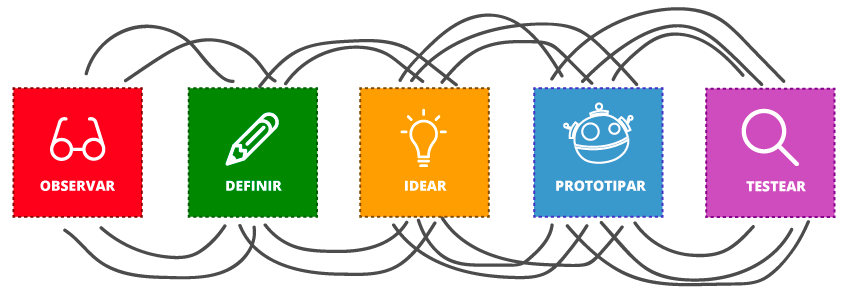
\includegraphics[scale=0.44]{designthinking}
    \centering
    \label{fig:Design Thinking}
\end{figure}

A lo largo del proceso se irá afinando ese contenido hasta desembocar en una solución que cumpla con los objetivos. Y seguramente, incluso los supere.

\textbf{Empatiza:} El proceso de Design Thinking comienza con una profunda comprensión de las necesidades de los usuarios implicados en la solución que estemos desarrollando, y también de su entorno. Debemos ser capaces de ponernos en la piel de dichas personas para ser capaces de generar soluciones consecuentes con sus realidades.

Algunas técnicas: \textbf{Entrevistas, Inmersión Cognitiva, Focus Group.}

\textbf{Define:} Durante la etapa de Definición, debemos cribar la información recopilada durante la fase de Empatía y quedarnos con lo que realmente aporta valor y nos lleva al alcance de nuevas perspectivas interesantes. Identificaremos problemas cuyas soluciones serán clave para la obtención de un resultado innovador.

Algunas técnicas: \textbf{Mapa de Empatía, User Personas, Listas de Problemas.}

\textbf{Idea:} La etapa de Ideación tiene como objetivo la generación de un sinfín de opciones. No debemos quedarnos con la primera idea que se nos ocurra. En esta fase, las actividades favorecen el pensamiento expansivo y debemos eliminar los juicios de valor. A veces, las ideas más estrambóticas son las que generan soluciones visionarias.

Algunas técnicas: \textbf{Brainstorming, Product Box, MindMap.}

\textbf{Prototipa:} En la etapa de Prototipado volvemos las ideas realidad. Construir prototipos hace las ideas palpables y nos ayuda a visualizar las posibles soluciones, poniendo de manifiesto elementos que debemos mejorar o refinar antes de llegar al resultado final.

Algunas técnicas: \textbf{Sketches, WireFrames, Prototipo, StoryBoard.}

\textbf{Testea:} Durante la fase de Testeo, probaremos nuestros prototipos con los usuarios implicados en la solución que estemos desarrollando. Esta fase es crucial, y nos ayudará a identificar mejoras significativas, fallos a resolver, posibles carencias. Durante esta fase evolucionaremos nuestra idea hasta convertirla en la solución que estábamos buscando.

Algunas técnicas: \textbf{Pruebas de Usuario, Test de Usabilidad.}

\subsection{MVP: Diseñando la Propuesta de Valor}

Como se ha explicado la metodología \textbf{Lean Startup} se basa en el Circuito de feedback de información: \textbf{crear, medir, aprender}. Lo que lleva al proceso de \textbf{Aprendizaje validado.}

Para crear nuestra propuesta de valor se ha decidido complementar con prácticas de \textbf{Design Thinking}: Empatiza, Define, Idea, Prototipa y Testea.

La mezcla de estas dos metodologías se conoce cómo \textbf{Lean Design} aunque actualmente está en desarrollo. Para entender mejor donde encajan estas dos metodologías disponemos de este gráfico.

\begin{figure}[H] 
    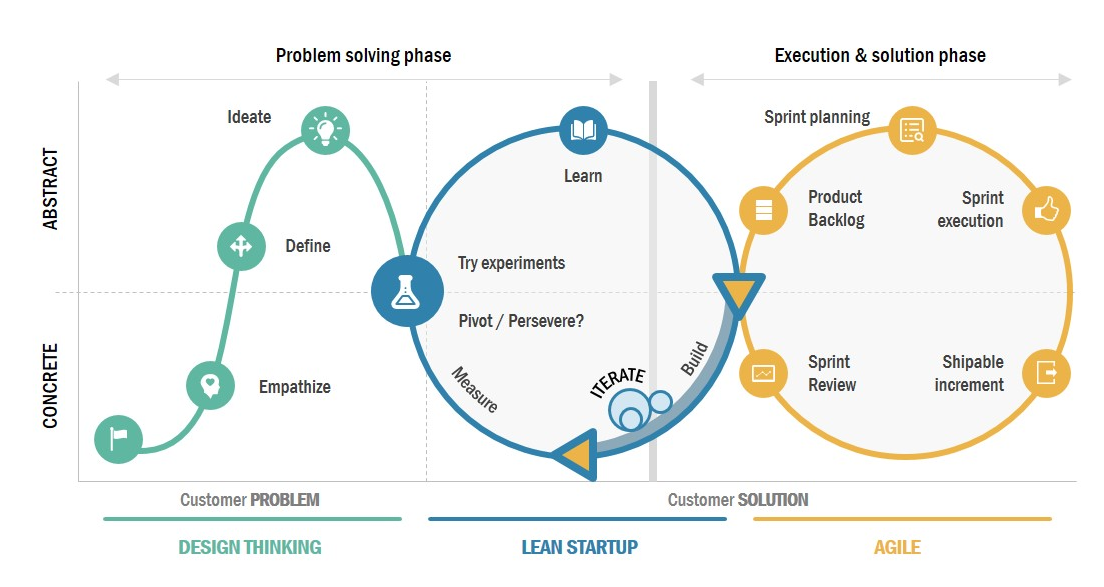
\includegraphics[scale=0.3]{leandesignagile}
    \centering
    \label{fig:Lean Design Agile}
    \caption{Diagrama de Lean Design}
\end{figure}

Con todo esto conseguimos un proceso que parte de la nada, se centra en el usuario, gestiona el caos, integra el error y es iterable.

Crear una \textbf{hipótesis}, diseñar un \textbf{experimento} para \textbf{testear} esa hipótesis, llevar a cabo el experimento, reunir datos, reflexionar y ver si validan o rechazan la hipótesis. Comenzamos:

\subsubsection{CREAR}

Lo primero de todo es definir nuestra \textbf{visión}. ¿Cuáles son nuestros objetivos?

El objetivo es conocer qué quieren los potenciales usuarios. Pero nos encontramos bajo unas condiciones de incertidumbre extrema. Nuestra tarea es diseñar para crear un nuevo producto o servicio bajo estas condiciones de incertidumbre extrema.

Es aquí donde necesitamos aplicar \textbf{Design Thinking:}

\textbf{EMPATIZAR}

Una forma de hacerlo podría ser \textbf{entrevistando} a los potenciales clientes para estar seguros de que el problema que queremos solventar existe.

En este caso el cliente más cercano es el propio \textbf{Manuel Rubio}. Así no diseñamos sobre hipótesis propias no validadas sino que lo hacemos teniendo en cuenta lo que es necesario para el usuario.

Tenemos varias reuniones por Teams en las que, cómo músico, me explica las dificultades por las que pasan a la hora de entrenar el oído y la importancia que el \textbf{entrenamiento auditivo} tiene.

\begin{figure}[H]
    \centering
    \includegraphics[scale=0.2]{MINDMAP0}
    \label{fig:Mindmap0}
    \caption{Ventajas del entrenamiento auditivo}
\end{figure}

Para entender mejor la situación necesito de un proceso de \textbf{investigación}. Internet es un inmenso campo de búsqueda de información. Por eso, paralelamente a las entrevistas busco información adicional que me permita entender mejor a nuestro usuario, el problema y cómo solucionarlo. Dado que mis conocimientos sobre música son básicos necesito de un estudio profundo de la teoría musical. 

Una vez entendido al usuario y sus necesidades, podemos pasar a definir el problema.

\textbf{DEFINIR}

El problema principal que se encuentran estos jóvenes músicos es la dificultad para entrenar el oído sumado a la dificultad para entrar en un conservatorio. Si quieren aprender a tocar por su cuenta no tienen los recursos necesarios para llevar a cabo este entrenamiento auditivo que Manuel nos ha explicado que es tan importante.

\textbf{IDEAR}

Por lo que vamos a intentar construir una solución que aporte valor. Para ello realizamos un pequeño MindMap donde nos enfocamos en los principales problemas y las posibles soluciones que podríamos llevar a cabo:

\begin{figure}[H]
    \centering
    \includegraphics[scale=0.37]{MINDMAP11}
    \label{fig:Mindmap1}
    \caption{MindMap Parte 1}
\end{figure}

\begin{figure}[H]
    \centering
    \includegraphics[scale=0.22]{MINDMAP2}
    \label{fig:Mindmap2}
    \caption{MindMap Parte 2}
\end{figure}
Después de varias iteraciones concluimos que una posible forma de solucionar estos problemas es mediante una WebApp con ejercicios de Entrenamiento Auditivo. 

\textbf{PROTOTIPAR}

Es ahora cuando toca llevar a cabo nuestra solución para testear esta hipótesis. 

Pero antes que nada debemos tener en cuenta nuestras limitaciones: poco tiempo para el desarrollo, aprender conceptos musicales, vamos a usar tecnologías que no conocemos. Y hacernos la pregunta: ¿Cuál es el \textbf{producto mínimo viable} (MVP) que puedo crear para obtener resultados?

Para ello, la técnica \textbf{MoSCoW} nos permitirá establecer las prioridades del proyecto. La cuál consiste en definir lo siguiente sobre la aplicación:

\textbf{Must have (Debe tener):} Características absolutamente críticas para el nuevo proyecto, sin ellas el proyecto es un fracaso.

\begin{compactitem}
    \item Modo Práctica
    \item Ejercicio Notas
    \item Ejercicio Intervalos
    \item Ejercicio Escalas
\end{compactitem}

\textbf{Should have (Debería incluir):} Aspectos del proyecto críticos también, pero no imprescindibles.

\begin{compactitem}
    \item Opciones personalizables
    \item Varios instrumentos
    \item Piano
    \item Responsive
\end{compactitem}

\textbf{Could have (Podría incluir):} Iniciativas que estaría bien tenerlas, ya que añadirían valor al proyecto, pero no son críticas.

\begin{compactitem}
    \item Ejercicio Acordes
    \item Ejercicio Ritmos
    \item Ejercicio Progresiones
\end{compactitem}

\textbf{Won’t have (No se van a hacer):} Características que no se merecen la inversión y no aportan ningún beneficio en este momento y se podrían considerar más tarde.

\begin{compactitem}
    \item Modo reto
    \item Modo nocturno
    \item Varios Idiomas
\end{compactitem}


Este MVP no debe ser perfecto, lo que queremos es aprender lo más rápido posible. Añadir características a nuestro producto que todavía ni sabemos cómo va a ser aceptado es una perdida de tiempo. Por lo que vamos a centrarnos en desarrollar prioritariamente lo que debe tener y más tarde lo que debería incluir.

Una vez establecidas las prioridades del proyecto pasamos a visualizarlas en forma de Sketches en papel, y más tarde realizamos los Wireframes teniendo en cuenta la filosofía de diseño Mobile First. Tratamos de realizar un diseño simple pero efectivo basado en tres columnas.
\begin{comment}
\begin{figure}[H]
    \centering
    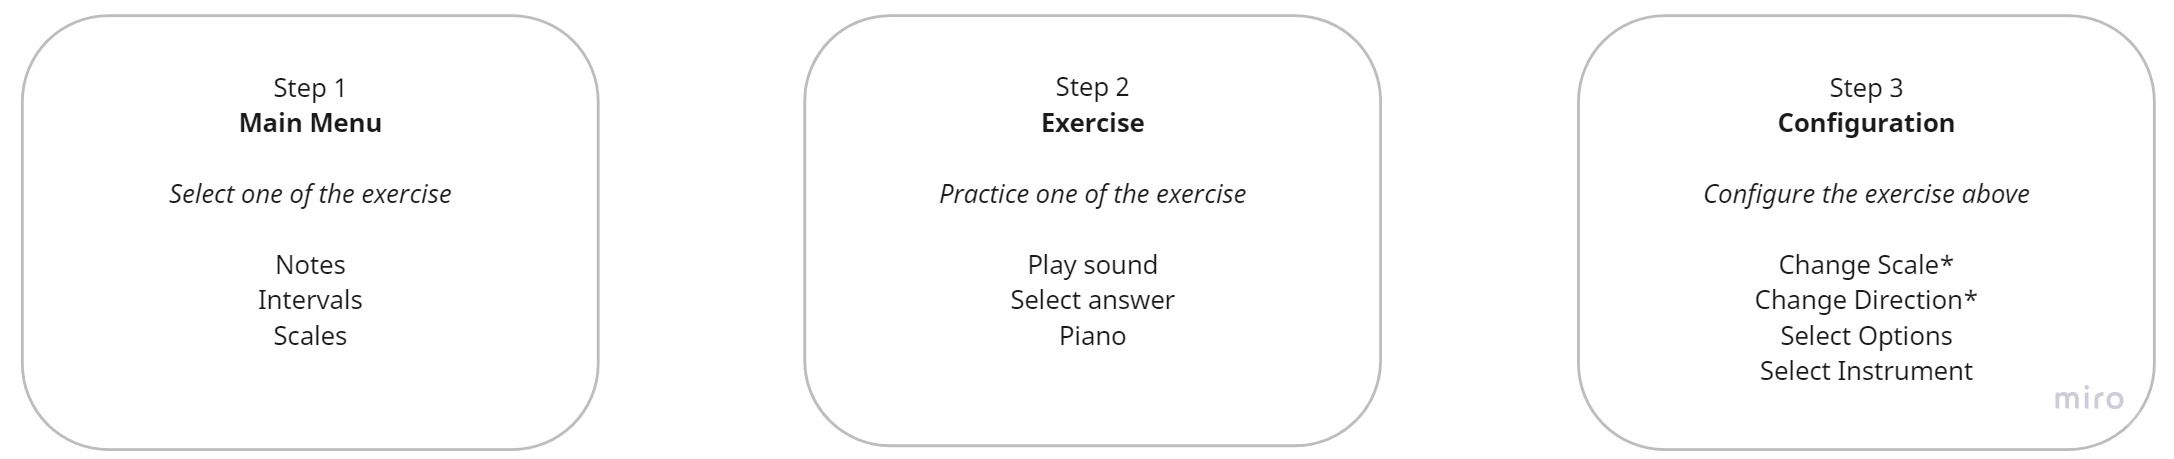
\includegraphics[scale=0.18]{WireframeSteps}
    \label{fig:WireframeSteps}
\end{figure}
\begin{figure}[H]
    \centering
    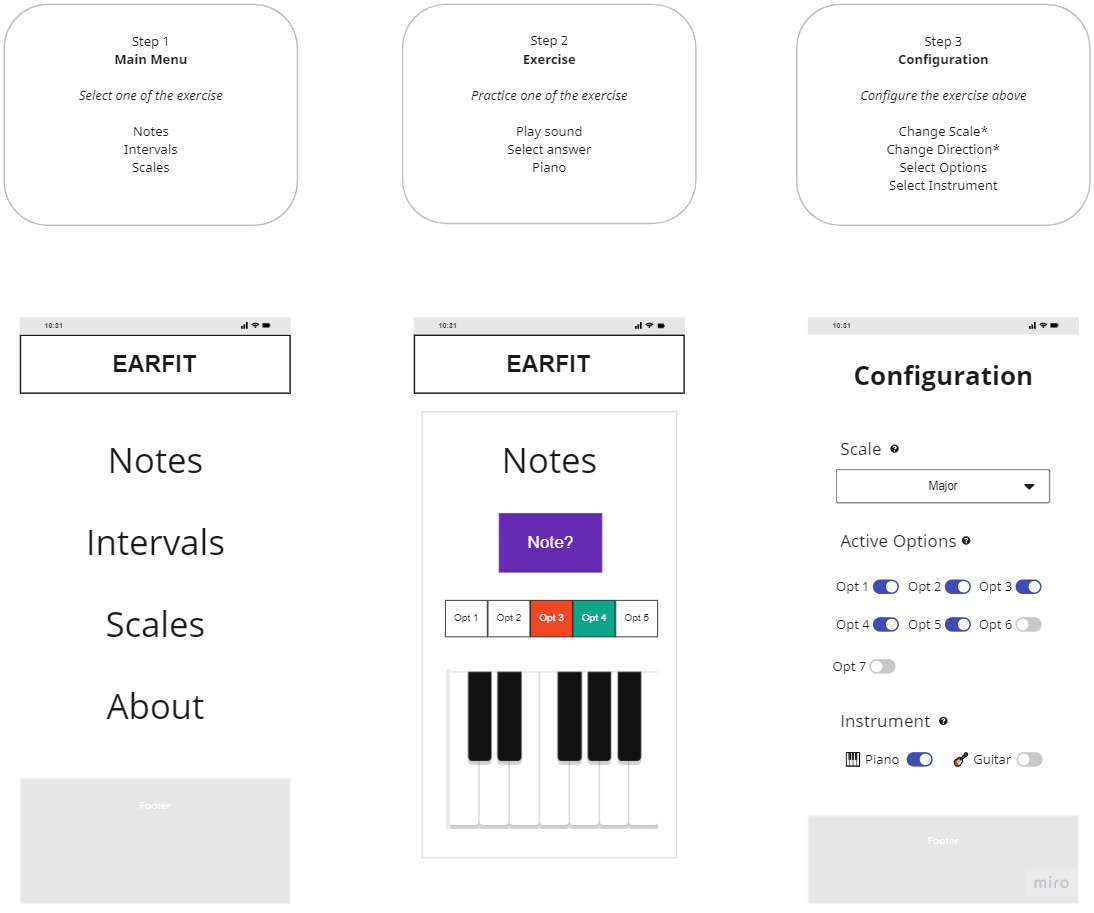
\includegraphics[scale=0.3]{Wireframes}
    \label{fig:Wireframe}
    \caption{Prototipo Smartphone}
\end{figure}
\end{comment}

\begin{figure}[H]
    \centering
    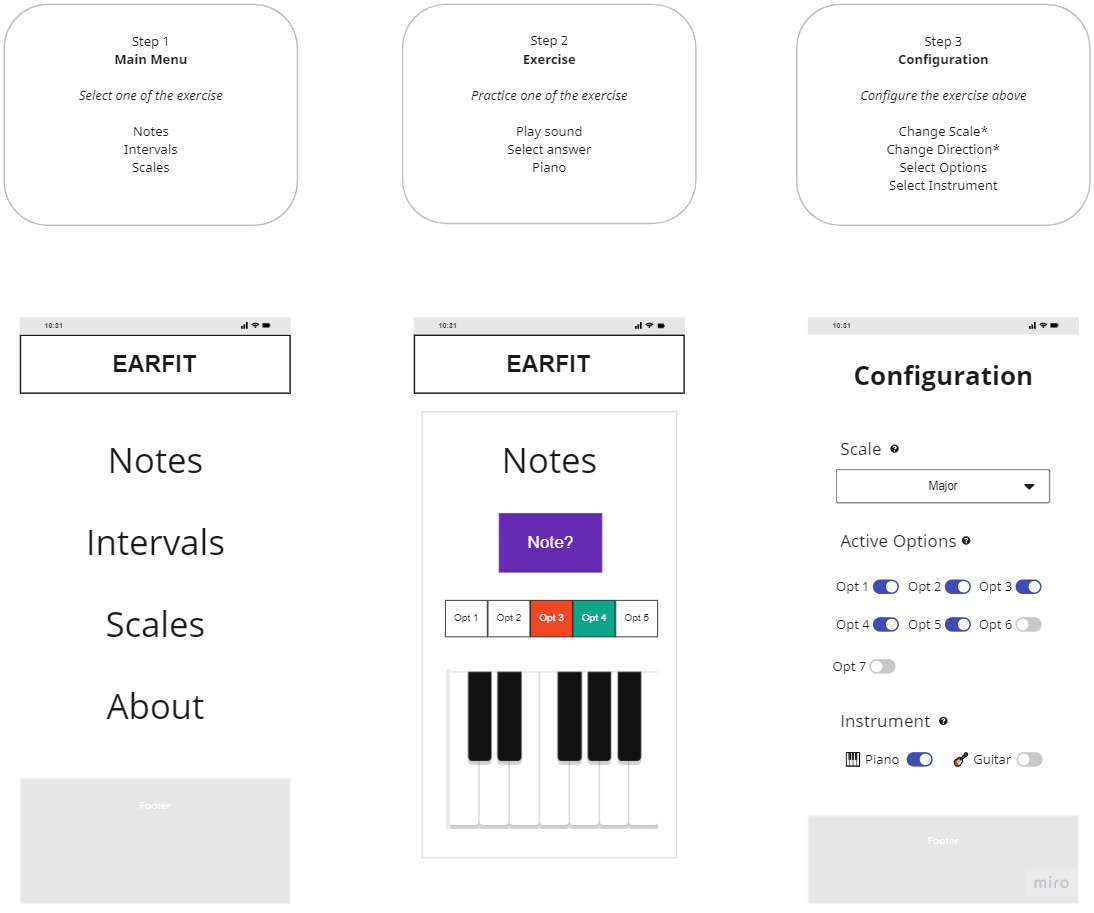
\includegraphics[scale=0.37]{Wireframes}
    \label{fig:Wireframes}
    \caption{Prototipo Smartphone}
\end{figure}

\begin{figure}[H]
    \centering
    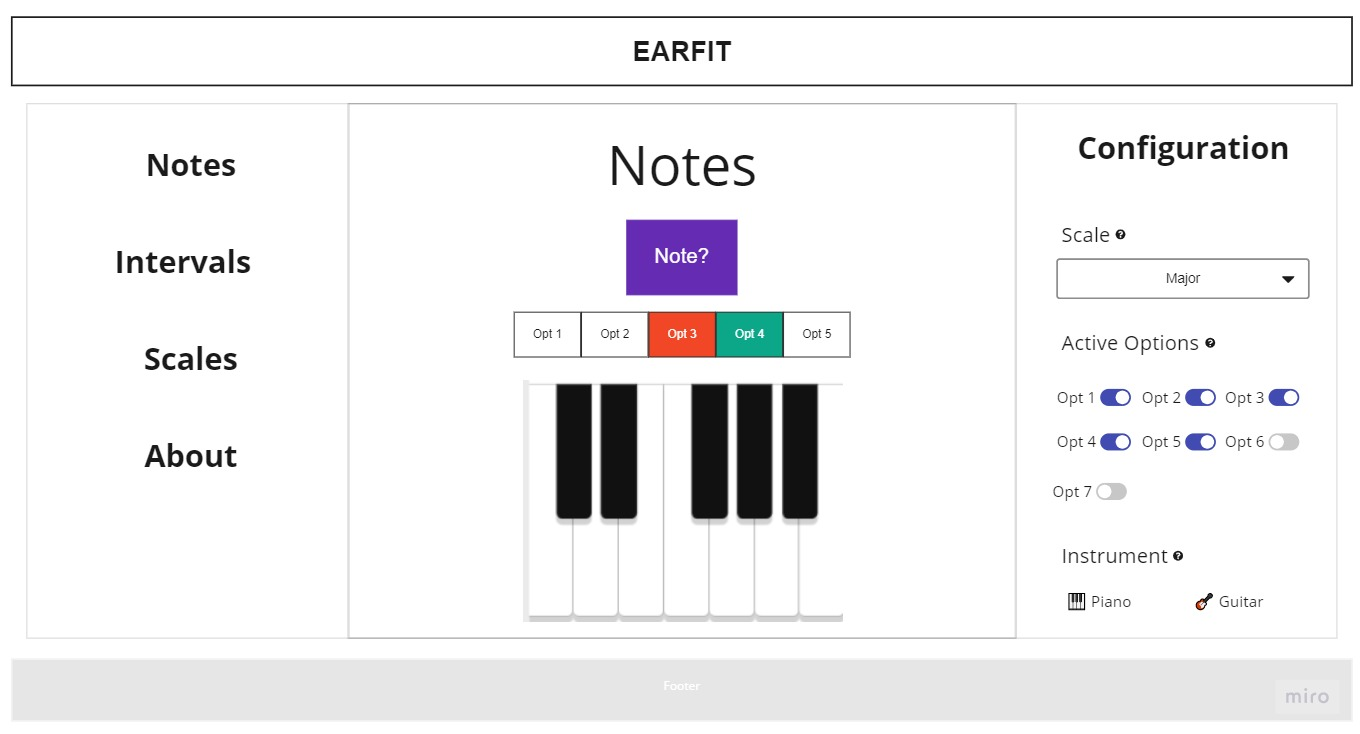
\includegraphics[scale=0.3]{WireframePC}
    \label{fig:WireframePC}
    \caption{Prototipo PC}
\end{figure}

La ventaja principal del uso de \textbf{prototipos en UX o Experiencia de Usuario} es que, ayudan a plasmar visualmente los objetivos y como se alinean con las expectativas y necesidades de los usuarios y si son satisfechas a través del producto diseñado.

Modificar un prototipo, tiene un coste menor que modificar el producto digital una vez subido a producción, por lo que supone también una ventaja en el ahorro de costes dentro del proceso de desarrollo.

Ayuda a que el cliente ya tenga una visión sobre parte del proyecto y que nos pueda proporcionar su feedback desde las fases tempranas.

\textbf{TESTEAR}

En esta fase, es importante que entendamos que no estamos vendiendo. Se trata de aprender del feedback del usuario para hacer posteriormente una nueva versión mejorada de nuestra solución.

Después de haber testeado los primeros diseños con el usuario, haber hecho correcciones y haber validado el último prototipo que hemos visto anteriormente, pasamos a crearlo usando \textbf{metodología Agile}.

En el siguiente capítulo se explicará esta metodología de trabajo seguida para implementar la solución. Y después de este los detalles técnicos de su desarrollo. Pero, por ahora seguimos con como fue el proceso de creación general.

\subsubsection{MEDIR}

Es hora de llevar a cabo el experimento, lo más común es poner los usuarios delante del producto y recoger así información sobre su comportamiento. Recoges los datos y reflexionas sobre ellos para \textbf{pivotar}, es decir, seguir adelante o cambiar de dirección. 

Lo importante es qué tan rápido puedes desarrollar tus experimentos para hacer evolucionar la aplicación. 

Los test fueron poco a poco en un proceso iterativo hasta llegar a completar los diseños del prototipo, generando siempre una versión entregable. Siguiendo la técnica del \textbf{Conserje}: empezando con un sólo usuario (Manuel Rubio) y una vez habiendo desarrollado la aplicación lo suficiente escalar y hacer pruebas con más usuarios.

La idea es ir implementando y testeando poco a poco la aplicación, empezando por los \textbf{Must haves} e ir añadiendo los \textbf{Should haves} paulatinamente y hacer ajustes según el feedback del usuario. Para dar respuesta a las siguientes preguntas:

¿Tiene la gente el problema que crees que tienen? ¿Realmente quieren lo que estas ofreciendo?

Para ello, cada vez que se desarrollaba una \textbf{nueva versión} de la aplicación. Se testeaba en una reunión con el tutor recogiendo \textbf{feedback} y haciendo los ajustes pertinentes. Más tarde se empezó a testear también con conocidos, en concreto dos estudiantes de conservatorio y una persona que está empezando a tocar. Es cuando se empezaron a aplicar algunas \textbf{métricas}:

Las que mejor se adecuaron a nuestro producto son: \textbf{Engagement} y \textbf{Tiempo en el producto} por usuario. También se tuvo en cuenta la \textbf{retención}: el usuario lo usa nuevamente, y la \textbf{referencia}: el usuario comparte el producto con sus amigos.

Además se utilizaron \textbf{test A/B}: enseñando dos versiones diferentes del producto al mismo tiempo para tomar decisiones acertadas. Aprovechando las características que nos ofrecía \textbf{Vercel} como veremos en su apartado.

Aclarar que aparte de estos test que \textbf{miden el éxito} de la aplicación se realizaron pruebas también relacionadas al funcionamiento cómo se verá más adelante en su apartado \textbf{Testing} en Desarrollo e Implementación.

\subsubsection{APRENDER}

Este proceso es necesario para mantenerse \textbf{ágiles} mientras crecemos. No invertir demasiado en grandes mejoras, sino hacer lotes de \textbf{pequeñas mejoras} más a menudo para aprender más. Lo que lleva a un circulo de interacción más rápido ya que puedes \textbf{detectar problemas} de calidad y tener mayor \textbf{feedback} sin tener que esperar a que el trabajo este hecho lo que propicia a que haya menos trabajo que rehacer.

\textbf{Lo que pudimos aprender} en este continuo proceso de crear, medir, aprender fue lo siguiente:

De los test con el \textbf{tutor} pudimos corregir lo siguiente:

En un principio no se incluían todos los \textbf{intervalos existentes}, sólo los de notas naturales, un test con el tutor nos hizo darnos cuenta de que faltaban las notas alteradas. Lo que llevo también a una investigación para corregir el nombre de estos, ya que descubrimos que dos intervalos con diferente nombre pueden sonar igual. Esto es debido a que los intervalos se nombran no sólo por la distancia de sus notas sino también por cómo están escritas en el pentagrama. Por ejemplo: entre Do y Dos hay 1 semitono y entre Do y Reb también hay 1 semitono, la misma distancia, suenan igual, pero son intervalos distintos.

También nos dió el feedback de que estaría bien añadir un \textbf{sonido al acertar}. Aprovechando el sonido de la misma respuesta para que así los usuarios puedan interiorizarla.

De los test con más \textbf{usuarios} pudimos mejorar lo siguiente:

En un principio se mostraban todas las opciones disponibles, lo que hacía el ejercicio muy difícil. Por lo que dejando como predeterminado tres opciones se ajustaba la \textbf{dificultad} inicial. Además descubrimos de que resultaba engorroso una vez señaladas varias opciones volver a seleccionarlas por lo que añadimos un botón que seleccionase y deseleccionase todas de golpe.

También descubrimos que había un problema de \textbf{compatibilidad} con iphone que hacía inservible la aplicación el cual pudimos corregir rápido. Así cómo poder ajustar el \textbf{volumen} de los sonidos ya que al principio no sonaba lo suficientemente alto.

De los \textbf{test A/B} lo siguiente:

Se mostraron dos versiones, una con \textbf{piano} en los ejercicios y otras sin él. Lo que pudimos observar es que las versiones con el piano generaban mayor \textbf{engagement} y \textbf{retención} por parte de los usuarios. Además los usuarios lo utilizaban para tener notas de referencia, lo que podía ayudar a la obtención de la respuesta correcta. Lo que en el ejercicio de notas resultó en una parte esencial.

Cómo se puede observar gracias a este proceso iterativo de crear, medir, aprender pudimos corregir fallos ágilmente y añadir funcionalidades que ni nos habíamos planteado en un primer momento gracias al feedback de los propios usuarios.

\subsubsection{CONCLUSIÓN}

Una vez pasado por todo este proceso iterativo, el resultado es un MVP que poder sacar al mercado. Y que se debe seguir mejorando. 

Los \textbf{Early Adopters}, los primeros en utilizar el producto no serán muy exigentes con la calidad pero esto es así con los nuevos clientes que vendrán más tarde. 

Todo se basa en un proceso de \textbf{Innovación Sostenida}, que se basaría en ir incrementando mejoras al producto ya existente.

Para ver capturas de la aplicación tras todo este proceso puedes ir al apartado \textbf{Resultado Final}

\section{Metodología de Trabajo}

Hablar de Agile brevemente

Scrum, como modelo organizativo  y DevOps como...

\subsection{Scrum}

\subsubsection{Kanban y Roadmap de Producto}

\subsection{DevOps}
\subsubsection{Integración Continua CI}
\subsubsection{Github}
\subsubsection{GitFlow}

\subsubsection{Despliegue Continuo CD}
\subsubsection{Github Actions}
\subsubsection{Vercel}

\section{Desarrollo e Implementación}

\subsection{Tecnologías Empleadas}

Comparativa Angular, React y Vue
https://unpocodejava.com/2018/12/21/react-vs-angular-vs-vue-js/

\subsubsection{VSCode}
\subsubsection{ESLint}
\subsubsection{Prettier}

\subsubsection{Next.js}

\subsubsection{TypeScript}

\subsubsection{Node.js}



\subsection{Implementación}

\subsubsection{Code Guidelines}
\subsubsection{Análisis y Diseño}
\subsubsection{Librerias Node.js}

\subsection{Testing}

Vercel Metricas

\subsubsection{Pruebas Unitarias}
\subsubsection{Evaluación de la Interfaz}

\section{Resultado Final}

Explicacion y capturas

\newpage

%%%%%%%%%%%%%%%%%%%%%%%%%%%%%% 4 Conclusiones %%%%%%%%%%%%%%%%%%%%%%%%%%%%%%%%%%%%%
\chapter{Conclusiones}

En este capítulo se detallan las conclusiones derivadas del TFG y la propuesta de posibles trabajos futuros.

Las citas del texto Autor \cite{giaquinta}, Autor \cite{fortune}, Autor \cite{fortuneB}, Autor \cite{mitchell} y Autor \cite{morrey} deben ir referenciadas en la bibliografia.


Qué he aprendidos
Qué debo mejorar

\blankpage



%%%%%%%%%%%%%%%%%%%%%%%%%%%%%%% Bibliografía %%%%%%%%%%%%%%%%%%%%%%%%%%%%%%%%%%%%%

\phantomsection
\addcontentsline{toc}{chapter}{Bibliografía}
\footnotesize{
%\bibliographystyle{hispa}
\bibliographystyle{IEEEtran}
\bibliography{bibliografia}
}
% No expandir elementos para llenar toda la página
\raggedbottom
\afterpage{\blankpage}
\newpage


%%%%%%%%%%%%%%%%%%%%%%%%%%%%%%% Apéndices %%%%%%%%%%%%%%%%%%%%%%%%%%%%%%%%%%%%%%%%

\appendix
\phantomsection
\addcontentsline{toc}{chapter}{Apéndices}
\mbox{}
\vfill
\begin{center}
\begin{Huge}
\textbf{Apéndices}
\end{Huge}
\end{center}
\vfill
\mbox{}
\thispagestyle{empty}
\newpage
\mbox{}
\thispagestyle{empty}
\newpage

%%%%%%%%%%%%%%%%%%%%%%%%%%%%%%% Conceptos Musicales %%%%%%%%%%%%%%%%%%%%%%%%%%%%%
\chapter{Conceptos Musicales}
\label{sec:apendice}

\section{Notas}

Sección del apéndice

\section{Intervalos}
\section{Escalas}






% Fin del documento
\end{document}
